\chapter{Test Results}
\label{cha:pierwszyDokument}

\section{First Set of Tests}

First set of tests uses historical data from 
Historical data from WSE (WIG20) of 3 stocks have been used.


For the first test historical data

\subsection{Trend Following}

\subsubsection{Short-term trend results}

\begin{figure}[H]
  \begin{center}
    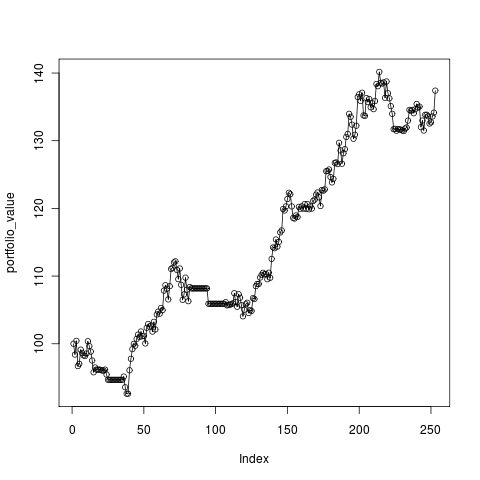
\includegraphics[scale=.4]{rplot0.png}
  \end{center}
  \caption{GA flow chart \cite{Haupt:2004:PGA:1007746}}
\end{figure}


\subsubsection{Intermediate-term trend results}

\begin{figure}[H]
  \begin{center}
    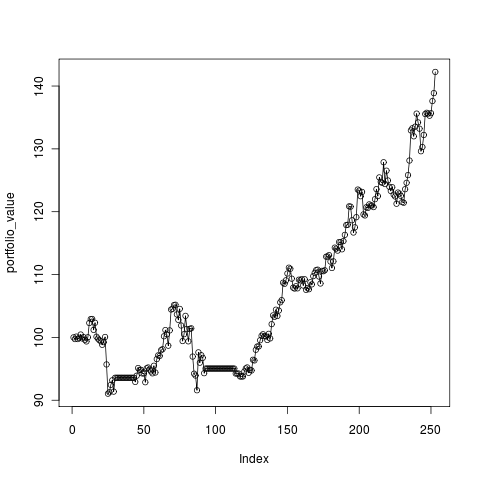
\includegraphics[scale=.4]{rplot.png}
  \end{center}
  \caption{GA flow chart \cite{Haupt:2004:PGA:1007746}}
\end{figure}


%---------------------------------------------------------------------------

\subsection{Genetic Algorithm}

\begin{figure}[H]
  \begin{center}
    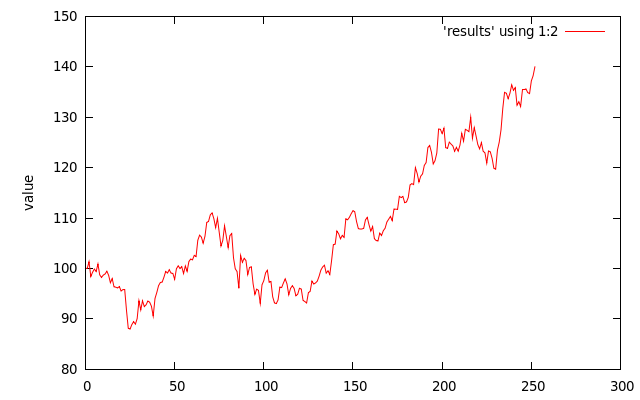
\includegraphics[scale=.5]{simple-genetic-algo.png}
  \end{center}
  \caption{GA flow chart \cite{Haupt:2004:PGA:1007746}}
\end{figure}


